\section{Traffic Censorship}
Censorship of Internet traffic occurs in a variety of forms all over the world. Most common is censorship of Web traffic (e.g., HTTP, DNS, and other TCP protocols related to browsing the Web). The most aggressive censorship takes place in countries where citizens' access to the Internet is very limited. Verkamp and Gupta \cite{Verkamp2012} conducted experiments to infer the mechanics of various countries' approaches to Web censorship and also provided a set of independent sources ranking countries based on the severity of their censorship. 

\begin{figure}[h]
\centering
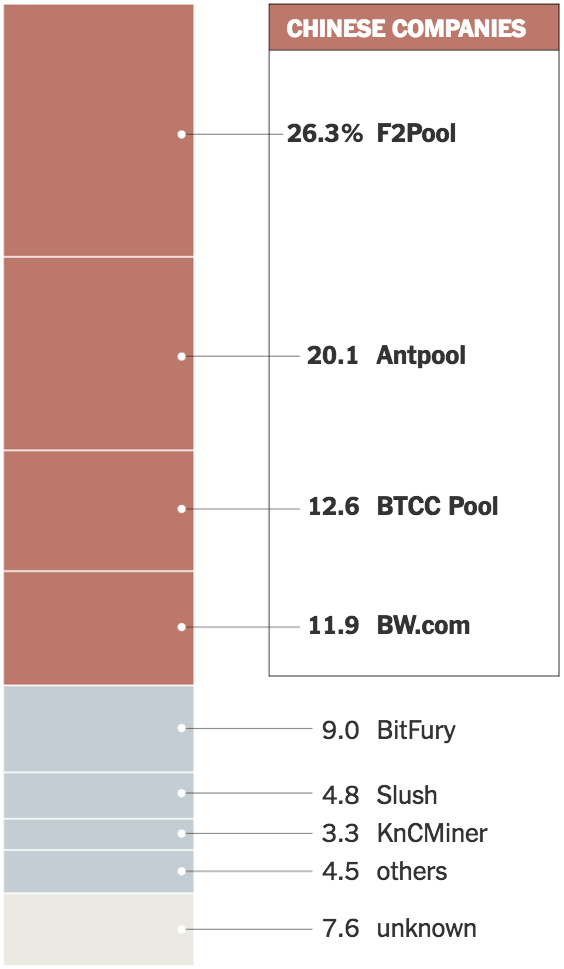
\includegraphics[height=250pt]{Images/NYT-Bitcoin-China.png}
\caption{From \cite{Popper2016}: the shares of mined Bitcoin blocks from May 24 to June 24, 2016 by mining pool.}
\label{fig:BTCPools}
\end{figure}

In our review of existing resesarch, four countries were repeatedly identified as the most severe censors: North Korea, Cuba, Iran, and China. Of these, China is the most interesting case for our purposes for two reasons: (1) its Internet-connected population far surpasses the others' and (2) it is a hotbed of Bitcoin mining activity, with Chinese-run mining pools accounting for an estimated 70\% of all Bitcoin mining power as of June 2016 (Figure~\ref{fig:BTCPools}). As a collection, China's censorship measures are colloquially referred to as The Great Firewall of China (GFW).
